\documentclass[Main]{subfiles}

\begin{document}

\section*{Part 1}
\paragraph{Implement the factorial function in Prolog.}

Implementing this function is seen in \codeTitle \ref{lst:part1}.
A factorial function works as the math function $N!$ which gives $N \cdot (N-1) \cdot (N-2) \cdot \ldots \cdot 1$.

First we create the base rule, \texttt{factorial(0, Res)}, which returns 1. 
At this point we will not look further down.

Then we create the recursive rule, \texttt{factorial(N,Res)}, which first checks if \texttt{N} is greater than 0, assign a new value to \texttt{N1}, runs the function recursive with the new value \texttt{N1}, and returns the product of the original value, \texttt{N}, and the result, \texttt{Res1}.

The value of the factorial function can be written with the function \texttt{fact(N)}, which calls the recursive function and writes the value.

\begin{lstlisting}[caption=Fatorial function in Prolog, style=Code-Prolog, label=lst:part1]
factorial(0,Res) :-
    Res is 1.

factorial(N,Res) :-
    N > 0,
    N1 is N-1,
    factorial(N1,Res1),
    Res is Res1*N.

fact(N) :-
	factorial(N, Val),
	writeln(Val).
\end{lstlisting}


\newpage
\section*{Part 2}
\paragraph{Demonstrate that your factorial function is correct for the numeric values between 1 and 10.}
To demonstrate that the function works, we find the first 10 values on \href{http://en.wikipedia.org/wiki/Factorial}{Wikipedia} and compare them to the output of the function:
\\
\\
\begin{minipage}{0.45\linewidth}
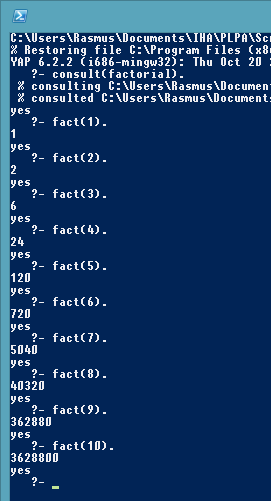
\includegraphics[scale=1]{Assi1}
\end{minipage}
\hspace{0.25cm}
\begin{minipage}{0.45\linewidth}

\begin{table}[H]
\centering
\begin{tabular}{cr}
\hline
N & N! \\ \hline
1 & 1 \\
2 & 2 \\
3 & 6 \\
4 & 24 \\
5 & 120 \\
6 & 720 \\
7 & 5040 \\
8 & 40320 \\
9 & 362880 \\
10 & 3628800 \\ \hline
\end{tabular}
\caption{Factorial of the first 10 integers}
\end{table}

\end{minipage}
\\
\\
As seen above the values are equal to what Wikipedia has described them to be.


\newpage
\section*{Part 3}
\paragraph{Draw a refutation for calculating the factorial of the value 3}

\begin{figure}[hbtp]
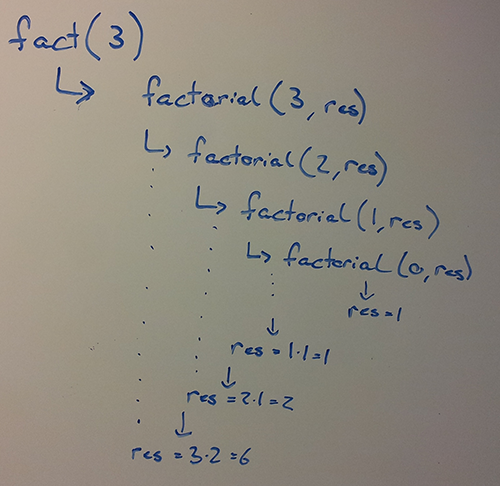
\includegraphics[width = 1\textwidth]{Assi1-draw}
\end{figure}










\end{document}